\section{Experimental Method}
\subsection{Data format}
For this work a specimen of $\gamma$-InSe was imaged using the momentum resolved electron energy loss technique in an energy filtered transmission electron microscope.
The file was supplied with aligned zero-loss peaks in Gatan's \textit{.dm4} format which had to be converted to a python object for further data processing in python, for the conversion from Gatan's proprietary file to a python object the excellent ncempy package \cite{ncempy} was used.\\

The measurement data is gathered by taking energy filtered diffraction images at different energy losses.
All these images are stacked corresponding to their energy loss value, resulting in a EFTEM image stack as illustrated in figure \ref{fig:eftem-stack}.
In the illustrated cube the horizontal planes or slices are diffraction mode images associated with an energy loss $\Delta E$, these energy slices have their own momentum axes that are not necessarily aligned with the whole stack.
After alignment the individual pixels in the EFTEM stack can be fully expressed by four values, three coordinates: $q_x$, $q_y$, $\Delta E$ and one scattering intensity $I$.\\

\begin{figure}
	\centering
	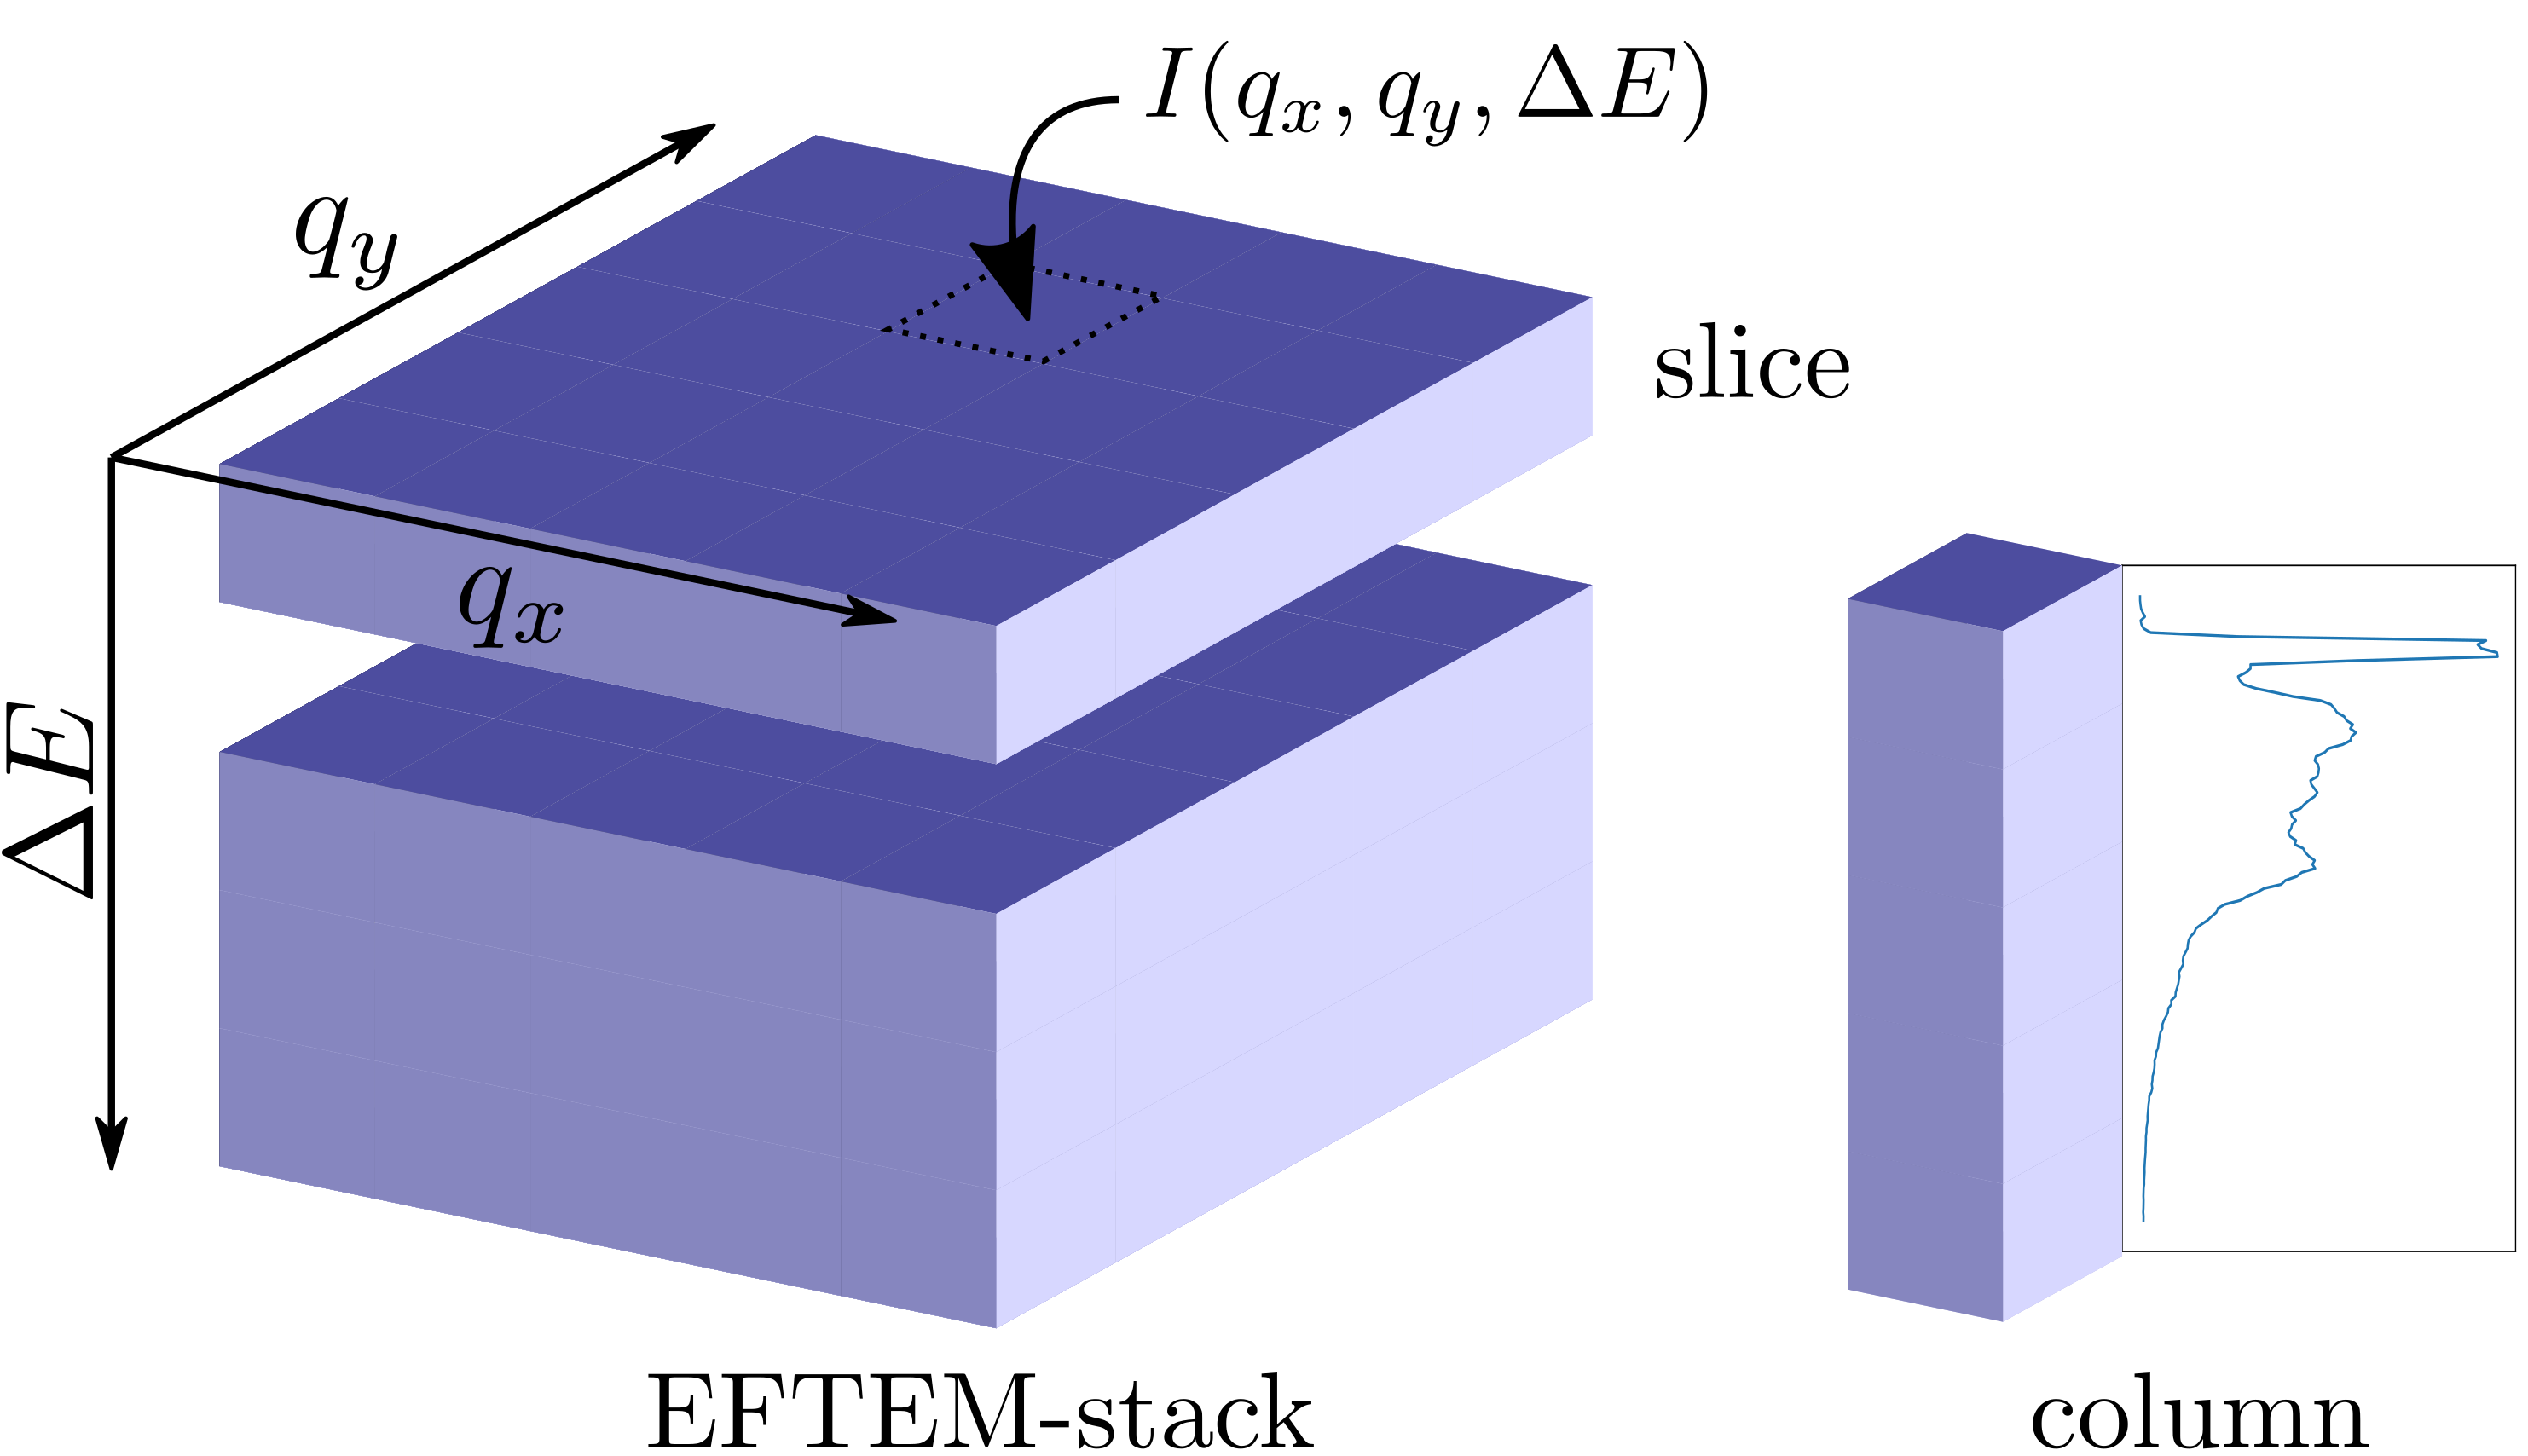
\includegraphics[width=0.75\linewidth, keepaspectratio]{eftem-stack.png}
	\caption{An illustration of an EFTEM-stack, slice, column and corresponding axes.}
	\label{fig:eftem-stack}
\end{figure}

An example of such a spectrum is illustrated in figure \ref{fig:spectrum}. Another way is to extract multiple of these columns such that their total momentum increases, doing this yields a energy-momentum map as pictured in figure \ref{fig:qmap}.
Once the EFTEM stack is aligned it is possible to start extracting sets of values in meaningful ways. One way is to take a single column from the top of the stack to the bottom, doing this results in a 1D-array of values for a set position in momentum space and varying energy-loss, this is called an electron energy loss spectrum.

\begin{figure}
	\centering
	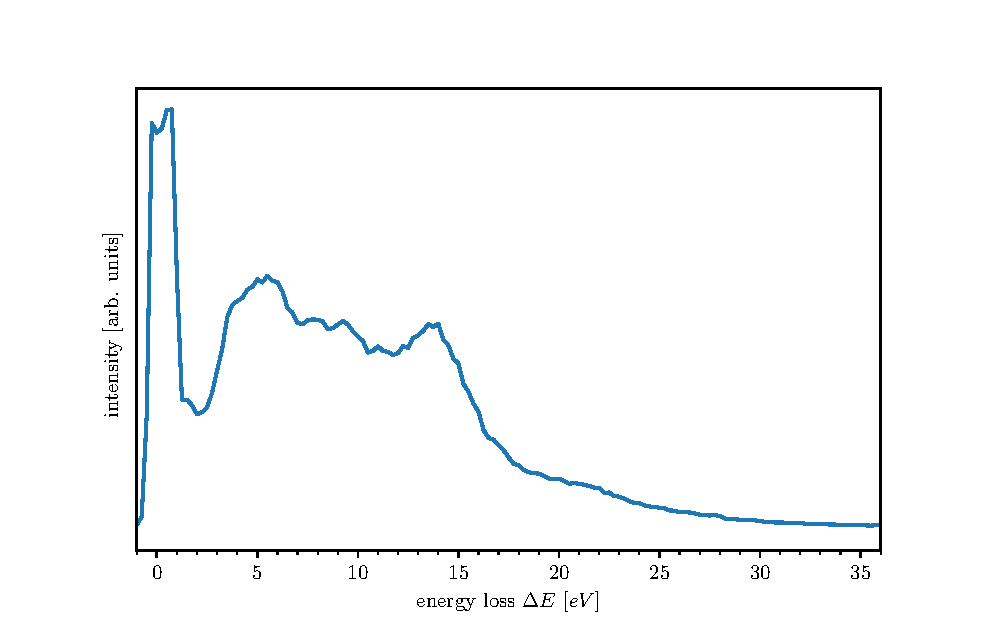
\includegraphics[width=0.5\linewidth, keepaspectratio]{big-spectrum.eps}
	\caption{EELS spectrum of $\gamma$-InSe for $q_{\perp}=0$}
	\label{fig:spectrum}
\end{figure}

\begin{figure}
	\centering
	\includegraphics[width=0.5\linewidth, keepaspectratio]{qmap-example.eps}
	\caption{q-EELS map of $\gamma$-InSe along $\Gamma \rightarrow M \rightarrow K$}
	\label{fig:qmap}
\end{figure}


\subsection{Data correction techniques}
\subsubsection{Removing/altering values}
Before any meaningful results can be extracted from the EFTEM stack it is important to first correct the data.
This process starts by removing all the values corresponding to negative energy losses, these values are can be incorrectly indexed as a result of the microscope software aligning the slices such that the zero-loss peak is at an energy loss of $0eV$.
It does this by shifting slices up or down to match them to their true energy loss, slices corresponding to negative energy losses are duplicates of slices at positive energy losses.\\
After removing the negative energy loss slices the negative intensity values are raised by the minimum amount needed to make all values positive.
This means that all values of the entire stack are raised by the absolute value of the most negative intensity. Doing this changes the performance of further techniques for the better.\\
Since the acquisition time of the EFTEM stack is quite large and not all slices are taken at the same time it might happen that the sample moves due to disturbances. Correcting this is done by convoluting a slice with Sobel matrices to get an edge-detected image, these images are then aligned by means of Fourier phase correlation \cite{Sjodahl:93}.

\subsubsection{Zero-loss peak and Batson correction}
To try and remove the zero-loss peak of the q-EELS spectrum a Batson correction is performed. A Batson correction normally uses the sum of all EELS spectra in an EFTEM image of the sample to try and correct plural scattering and subtract the zero-loss peak \cite{PhysRevB.27.5224}. Since such an image was not available the sum of all q-EELS spectra in the first Brillouin zone was used since this region was more likely to correspond to a true image of the sample, the sum of the q-EELS spectra in the first Brillouin zone is called the correction spectrum.
The Batson correction is then performed by scaling the correction spectrum for each q-EELS spectra to be corrected in such a way that the integrated intensity of the zero-loss peaks matches, then the "centre of intensity" of the zero-loss peaks is determined and the correction spectrum is subtracted from the to be corrected q-EELS spectra with the centres of intensity aligned.

\subsection{Data processing techniques}
Since the EFTEM data is essentially a 3D cube of values it needs to be processed in such a way that the information it contains can be extracted. This is something that can not be done with the cube itself since it is hard to represent 3D data in meaningful ways.

\subsubsection{Integration techniques}
To achieve the goal of representing the data in a meaningful ways two integration techniques have been implemented in Python.
A radial integration method that finds the centre of the image stack which is determined to be the brightest pixel of the unaltered EFTEM stack since this is most probably the zero-loss peak at the centre of the unscattered beam.
From this centre outward the method sums all EELS spectra in circle from a certain radius to that radius plus a ringsize, the starting and ending radius as well as the ringsize can be specified by the user.
This method is the same as integrating with respect to the solid angle but without the appropriate constants involved
When this method is finished the result is an array of summed EELS spectra for a set of rings. This can be plotted as a momentum-energy EELS map as shown in \ref{fig:qmap}.
Instead of integration in circle segments over the entire stack the user might want to only do a line-like integration towards a single diffraction peak. If this is the case a similar method to the one described above is called except for the change that instead of circle segments in integrates over pie piece like segments.


\subsubsection{Slicing techniques}
Slicing refers to the term of "array slicing" in Python/Numpy which is the built-in way to select data from an array whose position in the array satisfies a condition. The slicing technique allows the user to specify one or two points and extracts all columns along the line between the two points. If one point is specified by the user the other point will be the centre of the EFTEM stack. This method returns an array of all the EELS spectra for the points along the line. This can again be plotted as a momentum-energy map.

\subsection{Data extraction}
Once the full 3D EFTEM stack is reduced to useful momentum-energy maps or $q$-EELS spectra it is possible to start identifying interesting features such as peaks in the $q$-EELS spectra at certain regions or bright spots in the momentum-energy maps. For instance, if long bright streaks can be observed in the momentum-energy map they might hint at a relation between energy and momentum of an often occurring reaction. One of such bright peaks that will be tracked is the plasmon peak at roughly $14.5eV$ energy loss.

